% =========================================================================
% BÀI 03: NHIỀU HƠN, ÍT HƠN, BẰNG NHAU (CHỦ ĐỀ 1 - LỚP 1)
% TOÀN BỘ CÂU HỎI ĐƯỢC VẼ HÌNH MINH HỌA TRỰC QUAN 100% BẰNG TIKZ
% =========================================================================

% --- CÁC HÀM VẼ ĐỒ VẬT, CON VẬT TRỰC QUAN CHO HỌC SINH LỚP 1 ---
\newcommand{\VeBanNho}[3][blue!70]{% #1=màu áo, #2=x, #3=y
  \begin{scope}[shift={(#2,#3)}, scale=0.62]
    \fill[orange!22] (0, 0.55) circle (0.24cm);
    \fill[brown!80!black] (-0.24,0.6) arc (180:0:0.24cm) -- cycle;
    \fill[black] (-0.08,0.56) circle (0.03cm);
    \fill[black] (0.08,0.56) circle (0.03cm);
    \draw[line width=0.6pt, red!70!black] (-0.06,0.48) arc (-150:-30:0.08cm);
    \fill[#1] (-0.18,0.1) rectangle (0.18,0.38);
    \draw[line width=1.4pt, blue!90!black] (-0.09,0.1) -- (-0.09,-0.15);
    \draw[line width=1.4pt, blue!90!black] (0.09,0.1) -- (0.09,-0.15);
  \end{scope}
}

\newcommand{\VeQuaTao}[2]{% #1=x, #2=y
  \begin{scope}[shift={(#1,#2)}, scale=0.65]
    \fill[red!85!black] (-0.11,0.08) circle (0.22cm);
    \fill[red!85!black] (0.11,0.08) circle (0.22cm);
    \fill[red!85!black] (0,-0.05) circle (0.24cm);
    \draw[line width=1pt, brown!80!black] (0,0.24) to[out=70,in=-110] (0.06,0.42);
    \fill[green!70!black] (0.05,0.36) to[out=20,in=160] (0.24,0.42) to[out=-120,in=-20] cycle;
  \end{scope}
}

\newcommand{\VeQuaLe}[2]{% #1=x, #2=y
  \begin{scope}[shift={(#1,#2)}, scale=0.65]
    \fill[lime!75!black] (0,0.12) circle (0.16cm);
    \fill[lime!75!black] (0,-0.08) circle (0.24cm);
    \draw[line width=1pt, brown!80!black] (0,0.26) to[out=70,in=-110] (0.06,0.42);
    \fill[green!70!black] (0.05,0.36) to[out=20,in=160] (0.22,0.4) to[out=-120,in=-20] cycle;
  \end{scope}
}

\newcommand{\VeChiecO}[3][cyan!70!blue]{% #1=màu dù, #2=x, #3=y
  \begin{scope}[shift={(#2,#3)}, scale=0.68]
    \fill[#1] (-0.45,0.15) arc (180:0:0.45cm) -- cycle;
    \draw[line width=1.1pt, gray!80!black] (0,0.58) -- (0,-0.18) arc (0:-180:0.09cm);
    \fill[gray!80!black] (-0.03,0.58) rectangle (0.03,0.65);
  \end{scope}
}

\newcommand{\VeBongHoa}[3][magenta!80!red]{% #1=màu cánh, #2=x, #3=y
  \begin{scope}[shift={(#2,#3)}, scale=0.65]
    \draw[line width=1.1pt, green!60!black] (0,0) -- (0,-0.4);
    \fill[green!60!black] (0,-0.22) to[out=30,in=150] (0.18,-0.2) to[out=-120,in=-30] cycle;
    \foreach \a in {0,72,144,216,288} {
      \fill[#1] (\a:0.16) circle (0.1cm);
    }
    \fill[yellow!90!orange] (0,0) circle (0.08cm);
  \end{scope}
}

\newcommand{\VeChuChim}[2]{% #1=x, #2=y
  \begin{scope}[shift={(#1,#2)}, scale=0.55]
    \fill[cyan!80!blue] (0,0.2) circle (0.26cm);
    \fill[cyan!60!black] (-0.1,0.18) ellipse (0.16cm and 0.1cm);
    \fill[cyan!80!blue] (0.16,0.38) circle (0.17cm);
    \fill[white] (0.22,0.42) circle (0.05cm);
    \fill[black] (0.23,0.42) circle (0.03cm);
    \fill[orange!95!black] (0.32,0.38) -- (0.24,0.34) -- (0.24,0.42) -- cycle;
    \draw[line width=1pt, orange!90!black] (-0.06,-0.05) -- (-0.06,-0.2);
    \draw[line width=1pt, orange!90!black] (0.06,-0.05) -- (0.06,-0.2);
  \end{scope}
}

\newcommand{\VeChiecMu}[3][red!80!black]{% #1=màu mũ, #2=x, #3=y
  \begin{scope}[shift={(#2,#3)}, scale=0.65]
    \fill[#1] (-0.28,0) arc (180:0:0.28cm) -- cycle;
    \draw[line width=1.8pt, #1] (-0.38,0) -- (0.38,0);
  \end{scope}
}

\newcommand{\VeChuMeo}[2]{% #1=x, #2=y
  \begin{scope}[shift={(#1,#2)}, scale=0.62]
    \fill[orange!85!black] (0,0.18) circle (0.26cm);
    \fill[orange!85!black] (-0.22,0.32) -- (-0.12,0.54) -- (-0.02,0.4) -- cycle;
    \fill[pink!70] (-0.19,0.34) -- (-0.12,0.48) -- (-0.05,0.39) -- cycle;
    \fill[orange!85!black] (0.22,0.32) -- (0.12,0.54) -- (0.02,0.4) -- cycle;
    \fill[pink!70] (0.19,0.34) -- (0.12,0.48) -- (0.05,0.39) -- cycle;
    \fill[black] (-0.09,0.22) circle (0.032cm);
    \fill[black] (0.09,0.22) circle (0.032cm);
    \fill[pink!80!black] (0,0.14) circle (0.028cm);
    \draw[line width=0.5pt, gray!70!black] (-0.07,0.14) -- (-0.24,0.16);
    \draw[line width=0.5pt, gray!70!black] (-0.07,0.12) -- (-0.24,0.1);
    \draw[line width=0.5pt, gray!70!black] (0.07,0.14) -- (0.24,0.16);
    \draw[line width=0.5pt, gray!70!black] (0.07,0.12) -- (0.24,0.1);
  \end{scope}
}

\newcommand{\VeConCa}[2]{% #1=x, #2=y
  \begin{scope}[shift={(#1,#2)}, scale=0.65]
    \fill[cyan!75!blue] (0,0) ellipse (0.3cm and 0.17cm);
    \fill[cyan!75!blue] (-0.26,0) -- (-0.42,0.15) -- (-0.42,-0.15) -- cycle;
    \fill[white] (0.13,0.05) circle (0.045cm);
    \fill[black] (0.15,0.05) circle (0.025cm);
  \end{scope}
}

\newcommand{\VeChiecGhe}[2]{% #1=x, #2=y
  \begin{scope}[shift={(#1,#2)}, scale=0.62]
    \draw[line width=1.4pt, brown!80!black] (-0.24,-0.38) -- (-0.24,0.42);
    \draw[line width=1.4pt, brown!80!black] (0.24,-0.38) -- (0.24,0);
    \draw[line width=2.4pt, brown!80!black] (-0.28,0) -- (0.28,0);
    \draw[line width=1.3pt, brown!80!black] (-0.24,0.14) -- (0.24,0.14);
    \draw[line width=1.3pt, brown!80!black] (-0.24,0.32) -- (0.24,0.32);
  \end{scope}
}

\newcommand{\VeDauTay}[2]{% #1=x, #2=y
  \begin{scope}[shift={(#1,#2)}, scale=0.62]
    \fill[red!85!black] (-0.2,0.08) .. controls (-0.2,-0.18) and (-0.05,-0.32) .. (0,-0.36) .. controls (0.05,-0.32) and (0.2,-0.18) .. (0.2,0.08) -- cycle;
    \fill[green!70!black] (-0.18,0.08) -- (0,0.2) -- (0.18,0.08) -- (0,0.12) -- cycle;
    \fill[yellow!90!black] (-0.07,-0.04) circle (0.02cm);
    \fill[yellow!90!black] (0.07,-0.04) circle (0.02cm);
    \fill[yellow!90!black] (0,-0.18) circle (0.02cm);
  \end{scope}
}

\newcommand{\VeCocNuoc}[2]{% #1=x, #2=y
  \begin{scope}[shift={(#1,#2)}, scale=0.62]
    \draw[line width=1.2pt, cyan!70!blue] (-0.2,0.28) -- (-0.14,-0.22) -- (0.14,-0.22) -- (0.2,0.28);
    \fill[cyan!30] (-0.18,0.14) -- (-0.14,-0.2) -- (0.14,-0.2) -- (0.18,0.14) -- cycle;
  \end{scope}
}

\newcommand{\VeChiecThia}[2]{% #1=x, #2=y
  \begin{scope}[shift={(#1,#2)}, scale=0.62]
    \fill[gray!50] (0,0.18) ellipse (0.13cm and 0.2cm);
    \draw[line width=1.6pt, gray!70] (0,0.05) -- (0,-0.32);
  \end{scope}
}

\newcommand{\VeChuOng}[2]{% #1=x, #2=y
  \begin{scope}[shift={(#1,#2)}, scale=0.62]
    \fill[yellow!90!orange] (0,0) ellipse (0.22cm and 0.15cm);
    \draw[line width=1.1pt, black] (-0.06,-0.14) -- (-0.06,0.14);
    \draw[line width=1.1pt, black] (0.06,-0.14) -- (0.06,0.14);
    \fill[cyan!20, draw=cyan!70!black, line width=0.4pt] (-0.05,0.1) ellipse (0.11cm and 0.16cm);
    \fill[cyan!20, draw=cyan!70!black, line width=0.4pt] (0.05,0.1) ellipse (0.11cm and 0.16cm);
    \fill[black] (0.16,0.04) circle (0.025cm);
  \end{scope}
}

\newcommand{\VeChuBuom}[2]{% #1=x, #2=y
  \begin{scope}[shift={(#1,#2)}, scale=0.62]
    \fill[purple!70!blue] (-0.16,0.12) ellipse (0.18cm and 0.12cm);
    \fill[purple!70!blue] (0.16,0.12) ellipse (0.18cm and 0.12cm);
    \fill[purple!60!pink] (-0.14,-0.08) ellipse (0.14cm and 0.09cm);
    \fill[purple!60!pink] (0.14,-0.08) ellipse (0.14cm and 0.09cm);
    \fill[black] (0,0) ellipse (0.04cm and 0.2cm);
    \draw[line width=0.6pt, black] (0,0.18) to[out=60,in=-60] (0.08,0.32);
    \draw[line width=0.6pt, black] (0,0.18) to[out=120,in=-120] (-0.08,0.32);
  \end{scope}
}

% =========================================================================
% PHẦN 1: TRẮC NGHIỆM LỰA CHỌN (12 CÂU)
% =========================================================================
\textbf{Phần 1. Trắc nghiệm lựa chọn (Học sinh quan sát hình và chọn đáp án đúng)}
\setcounterpageref{ex}{0}

% --- CÂU 1 ---
\begin{ex} %[1D1N03]
Quan sát hàng thỏ và hàng củ cà rốt dưới đây. Em thấy số thỏ và số cà rốt như thế nào?
\begin{center}
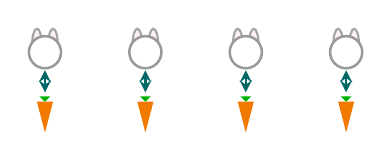
\begin{tikzpicture}[scale=0.85, baseline=(current bounding box.center)]
  \foreach \x in {-2.25, -0.75, 0.75, 2.25} {
    \draw[fill=pink!20, draw=gray!70, line width=0.8pt] (\x-0.12, 0.45) ellipse (0.07cm and 0.22cm);
    \draw[fill=pink!20, draw=gray!70, line width=0.8pt] (\x+0.12, 0.45) ellipse (0.07cm and 0.22cm);
    \draw[fill=white, draw=gray!80, line width=0.9pt] (\x, 0.32) circle (0.24cm);
    \draw[<->, >=stealth, dashed, line width=0.9pt, teal!80!black] (\x, 0.05) -- (\x, -0.28);
    \fill[orange!95!black] (\x-0.12, -0.42) -- (\x+0.12, -0.42) -- (\x, -0.88) -- cycle;
    \fill[green!70!black] (\x, -0.42) -- (\x-0.08, -0.34) -- (\x+0.08, -0.34) -- cycle;
  }
\end{tikzpicture}
\end{center}
\choice
{\True Bằng nhau}
{Thỏ nhiều hơn cà rốt}
{Thỏ ít hơn cà rốt}
{Không so sánh được}
\loigiai{
Mỗi chú thỏ được nối tương ứng với một củ cà rốt. Cả hai hàng đều có $4$ hình ($4 = 4$).\\
Vậy số thỏ và số cà rốt \textbf{bằng nhau}.\\
\textbf{Đáp án của câu hỏi là A}
}
\end{ex}

% --- CÂU 2 ---
\begin{ex} %[1D1N03]
Quan sát hình vẽ bông hoa và chú bướm dưới đây. Khẳng định nào sau đây đúng?
\begin{center}
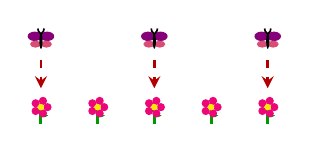
\begin{tikzpicture}[scale=0.8, baseline=(current bounding box.center)]
  \foreach \x in {-1.8, 0, 1.8} {
    \VeChuBuom{\x}{0.6}
    \draw[->, >=stealth, dashed, line width=0.9pt, red!70!black] (\x, 0.3) -- (\x, -0.15);
  }
  \foreach \x in {-1.8, -0.9, 0, 0.9, 1.8} {
    \VeBongHoa{\x}{-0.45}
  }
\end{tikzpicture}
\end{center}
\choice
{Số hoa ít hơn số bướm}
{Số hoa bằng số bướm}
{\True Số hoa nhiều hơn số bướm}
{Số bướm nhiều hơn số hoa}
\loigiai{
Có 3 chú bướm và 5 bông hoa. Vì $5 > 3$ nên \textbf{số hoa nhiều hơn số bướm}.\\
\textbf{Đáp án của câu hỏi là C}
}
\end{ex}

% --- CÂU 3 ---
\begin{ex} %[1D1H03]
Quan sát hình vẽ chiếc chén và chiếc đĩa dưới đây:
\begin{center}
\begin{tabular}{cc}

\begin{tikzpicture}[scale=0.8]
  \draw[fill=cyan!10, draw=blue!70, line width=1.2pt, rounded corners=4pt] (-1.8,-0.5) rectangle (1.8,0.7);
  \foreach \x in {-0.8, 0.8} {
    \draw[fill=cyan!30, draw=blue!80!black, line width=1.1pt] (\x-0.4, 0.45) -- (\x+0.4, 0.45) -- (\x+0.25, -0.15) -- (\x-0.25, -0.15) -- cycle;
  }
\end{tikzpicture}
&
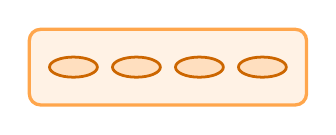
\begin{tikzpicture}[scale=0.8]
  \draw[fill=orange!10, draw=orange!70, line width=1.2pt, rounded corners=4pt] (-2.2,-0.5) rectangle (2.2,0.7);
  \foreach \x in {-1.5, -0.5, 0.5, 1.5} {
    \draw[fill=orange!25, draw=orange!80!black, line width=1pt] (\x, 0.1) ellipse (0.38cm and 0.16cm);
  }
\end{tikzpicture} \\[4pt]
{\bfseries\color{blue!90!black} 2 chiếc chén} & {\bfseries\color{orange!90!black} 4 chiếc đĩa}
\end{tabular}
\end{center}
Khẳng định nào sau đây đúng?
\choice
{Số chén nhiều hơn số đĩa}
{Số chén bằng số đĩa}
{Số đĩa ít hơn số chén}
{\True Số chén ít hơn số đĩa}
\loigiai{
Có 2 chiếc chén và 4 chiếc đĩa. Vì $2 < 4$ nên \textbf{số chén ít hơn số đĩa}.\\
\textbf{Đáp án của câu hỏi là D}
}
\end{ex}

% --- CÂU 4 ---
\begin{ex} %[1D1H03]
Hai tổ xếp thành hai hàng thẳng nhau như hình dưới đây:
\begin{center}
\begin{tikzpicture}[scale=0.85, baseline=(current bounding box.center)]
  \node[font=\bfseries\color{blue!80!black}, anchor=east] at (-2.4, 0.38) {Tổ Một (5 bạn):};
  \node[font=\bfseries\color{red!80!black}, anchor=east] at (-2.4, -0.42) {Tổ Hai (5 bạn):};
  \foreach \x in {-1.6, -0.8, 0, 0.8, 1.6} {
    \VeBanNho[blue!70]{\x}{0.35}
    \draw[<->, >=stealth, dashed, line width=0.8pt, gray!80] (\x, 0.1) -- (\x, -0.15);
    \VeBanNho[orange!85!black]{\x}{-0.4}
  }
\end{tikzpicture}
\end{center}
Số bạn của hai tổ là
\choice
{Tổ Một nhiều hơn}
{\True Bằng nhau}
{Tổ Hai nhiều hơn}
{Không biết}
\loigiai{
Mỗi bạn tổ Một đối diện với đúng một bạn tổ Hai, hai tổ đều có 5 bạn ($5 = 5$).\\
Vậy số bạn của hai tổ \textbf{bằng nhau}.\\
\textbf{Đáp án của câu hỏi là B}
}
\end{ex}

\newpage
% --- CÂU 5 ---
\begin{ex} %[1D1H03]
Quan sát ngôi sao ở Hình A và Hình B:
\begin{center}
\begin{tabular}{cc}
\begin{tikzpicture}[scale=0.8]
  \draw[fill=yellow!10, draw=orange!80, line width=1.2pt, rounded corners=4pt] (-1.8,-0.6) rectangle (1.8,0.6);
  \foreach \x/\y in {-1.1/0.25, 0/0.25, 1.1/0.25, -1.1/-0.25, 0/-0.25, 1.1/-0.25} {
    \node[draw=orange!80!black, fill=yellow!80, star, star points=5, star point ratio=2.2, line width=0.7pt, minimum size=0.55cm] at (\x,\y) {};
  }
\end{tikzpicture}
&
\begin{tikzpicture}[scale=0.8]
  \draw[fill=cyan!10, draw=blue!80, line width=1.2pt, rounded corners=4pt] (-1.5,-0.6) rectangle (1.5,0.6);
  \foreach \x/\y in {-0.7/0.25, 0.7/0.25, -0.7/-0.25, 0.7/-0.25} {
    \node[draw=blue!80!black, fill=cyan!60, star, star points=5, star point ratio=2.2, line width=0.7pt, minimum size=0.55cm] at (\x,\y) {};
  }
\end{tikzpicture} \\[4pt]
{\bfseries\color{orange!90!black} Hình A (6 ngôi sao)} & {\bfseries\color{blue!90!black} Hình B (4 ngôi sao)}
\end{tabular}
\end{center}
Khẳng định nào sau đây đúng?
\choice
{Hình A ít hơn hình B}
{Hình A bằng hình B}
{\True Hình A nhiều hơn hình B}
{Hình B nhiều hơn hình A}
\loigiai{
Hình A có 6 ngôi sao, Hình B có 4 ngôi sao. Vì $6 > 4$ nên \textbf{Hình A nhiều hơn hình B}.\\
\textbf{Đáp án của câu hỏi là C}
}
\end{ex}

% --- CÂU 6 ---
\begin{ex} %[1D1H03]
Quan sát số chú chim và số chiếc lồng chim:
\begin{center}
\begin{tikzpicture}[scale=0.85, baseline=(current bounding box.center)]
  \node[font=\bfseries\color{blue!80!black}, anchor=east] at (-2.3, 0.4) {3 chú chim:};
  \foreach \x in {-1.4, 0, 1.4} {
    \VeChuChim{\x}{0.35}
  }
  \node[font=\bfseries\color{brown!80!black}, anchor=east] at (-2.3, -0.45) {5 lồng chim:};
  \foreach \x in {-1.8, -0.9, 0, 0.9, 1.8} {
    \draw[fill=yellow!15, draw=brown!80!black, line width=1pt, rounded corners=2pt] (\x-0.3, -0.7) rectangle (\x+0.3, -0.2);
    \draw[brown!80!black, line width=0.6pt] (\x-0.1, -0.7) -- (\x-0.1, -0.2);
    \draw[brown!80!black, line width=0.6pt] (\x+0.1, -0.7) -- (\x+0.1, -0.2);
  }
\end{tikzpicture}
\end{center}
Khẳng định nào sau đây đúng?
\choice
{Số chim nhiều hơn số lồng}
{Số chim bằng số lồng}
{\True Số chim ít hơn số lồng}
{Số lồng ít hơn số chim}
\loigiai{
Có 3 chú chim và 5 lồng chim. Vì $3 < 5$ nên \textbf{số chim ít hơn số lồng}.\\
\textbf{Đáp án của câu hỏi là C}
}
\end{ex}

% --- CÂU 7 ---
\begin{ex} %[1D1H03]
Có 5 bạn nhỏ và 4 chiếc mũ. Mỗi bạn đội một chiếc mũ thì:
\begin{center}
\begin{tikzpicture}[scale=0.85, baseline=(current bounding box.center)]
  \node[font=\bfseries, anchor=east] at (-2.4, 0.4) {5 bạn nhỏ:};
  \foreach \x in {-1.6, -0.8, 0, 0.8, 1.6} {
    \VeBanNho[teal!80!black]{\x}{0.35}
  }
  \node[font=\bfseries, anchor=east] at (-2.4, -0.4) {4 chiếc mũ:};
  \foreach \x in {-1.6, -0.8, 0, 0.8} {
    \draw[<->, >=stealth, dashed, line width=0.8pt, gray] (\x, 0.08) -- (\x, -0.2);
    \VeChiecMu[red!85!black]{\x}{-0.35}
  }
  \node[font=\bfseries\Large\color{red!80!black}] at (1.6, -0.35) {?};
\end{tikzpicture}
\end{center}
\choice
{Đủ mũ cho các bạn}
{Thừa 1 chiếc mũ}
{Thừa 2 chiếc mũ}
{\True Thiếu 1 chiếc mũ}
\loigiai{
Có 5 bạn nhỏ mà chỉ có 4 chiếc mũ. Mỗi bạn một mũ thì còn 1 bạn chưa có mũ.\\
Vậy \textbf{thiếu 1 chiếc mũ}.\\
\textbf{Đáp án của câu hỏi là D}
}
\end{ex}

% --- CÂU 8 ---
\begin{ex} %[1D1V03]
Quan sát đĩa táo và đĩa lê dưới đây:
\begin{center}
\begin{tabular}{cc}
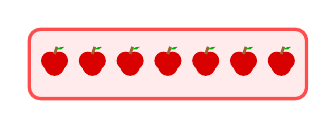
\begin{tikzpicture}[scale=0.8]
  \draw[fill=red!8, draw=red!70, line width=1.2pt, rounded corners=4pt] (-2.2,-0.5) rectangle (2.2,0.6);
  \foreach \x in {-1.8, -1.2, -0.6, 0, 0.6, 1.2, 1.8} {
    \VeQuaTao{\x}{0.05}
  }
\end{tikzpicture}
&
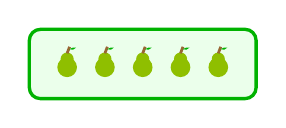
\begin{tikzpicture}[scale=0.8]
  \draw[fill=green!8, draw=green!70!black, line width=1.2pt, rounded corners=4pt] (-1.8,-0.5) rectangle (1.8,0.6);
  \foreach \x in {-1.2, -0.6, 0, 0.6, 1.2} {
    \VeQuaLe{\x}{0.05}
  }
\end{tikzpicture} \\[4pt]
{\bfseries\color{red!85!black} Đĩa A (7 quả táo)} & {\bfseries\color{green!70!black} Đĩa B (5 quả lê)}
\end{tabular}
\end{center}
Khẳng định nào sau đây đúng?
\choice
{Số quả lê nhiều hơn số quả táo}
{Số táo bằng số lê}
{Số quả táo ít hơn số quả lê}
{\True Số quả táo nhiều hơn số quả lê}
\loigiai{
Đĩa A có 7 quả táo, Đĩa B có 5 quả lê. Vì $7 > 5$ nên \textbf{số quả táo nhiều hơn số quả lê}.\\
\textbf{Đáp án của câu hỏi là D}
}
\end{ex}

\newpage
% --- CÂU 9 ---
\begin{ex} %[1D1V03]
Quan sát hai bình cá:
\begin{center}
\begin{tabular}{cc}
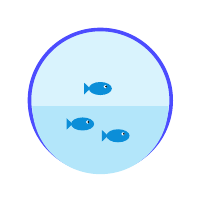
\begin{tikzpicture}[scale=0.75]
  \draw[fill=cyan!15, draw=blue!70, line width=1.3pt] (0,0) circle (1.2cm);
  \fill[cyan!30] (-1.15,-0.1) arc (180:360:1.15cm) -- cycle;
  \VeConCa{-0.3}{-0.4}
  \VeConCa{0.3}{-0.6}
  \VeConCa{0.0}{0.2}
\end{tikzpicture}
&
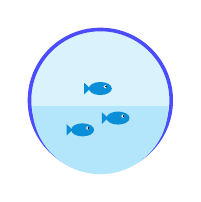
\begin{tikzpicture}[scale=0.75]
  \draw[fill=cyan!15, draw=blue!70, line width=1.3pt] (0,0) circle (1.2cm);
  \fill[cyan!30] (-1.15,-0.1) arc (180:360:1.15cm) -- cycle;
  \VeConCa{-0.3}{-0.5}
  \VeConCa{0.3}{-0.3}
  \VeConCa{0.0}{0.2}
\end{tikzpicture} \\[4pt]
{\bfseries\color{blue!90!black} Bình A (3 chú cá)} & {\bfseries\color{blue!90!black} Bình B (3 chú cá)}
\end{tabular}
\end{center}
Khẳng định nào đúng?
\choice
{\True Số cá ở hai bình bằng nhau}
{Bình A nhiều hơn bình B}
{Bình B nhiều hơn bình A}
{Không so sánh được}
\loigiai{
Cả hai bình đều có 3 chú cá ($3 = 3$).\\
Vậy \textbf{số cá ở hai bình bằng nhau}.\\
\textbf{Đáp án của câu hỏi là A}
}
\end{ex}

% --- CÂU 10 ---
\begin{ex} %[1D1V03]
Khung nào dưới đây có nhiều chấm tròn hơn?
\begin{center}
\begin{tabular}{cc}
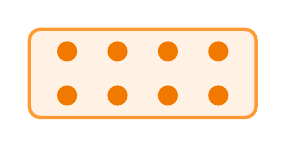
\begin{tikzpicture}[scale=0.8]
  \draw[fill=orange!10, draw=orange!80, line width=1.2pt, rounded corners=4pt] (-1.8,-0.7) rectangle (1.8,0.7);
  \foreach \x/\y in {-1.2/0.35, -0.4/0.35, 0.4/0.35, 1.2/0.35, -1.2/-0.35, -0.4/-0.35, 0.4/-0.35, 1.2/-0.35} {
    \fill[orange!95!black] (\x,\y) circle (0.16cm);
  }
\end{tikzpicture}
&
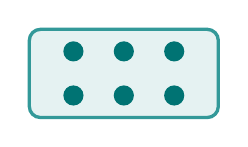
\begin{tikzpicture}[scale=0.8]
  \draw[fill=teal!10, draw=teal!80, line width=1.2pt, rounded corners=4pt] (-1.5,-0.7) rectangle (1.5,0.7);
  \foreach \x/\y in {-0.8/0.35, 0/0.35, 0.8/0.35, -0.8/-0.35, 0/-0.35, 0.8/-0.35} {
    \fill[teal!90!black] (\x,\y) circle (0.16cm);
  }
\end{tikzpicture} \\[4pt]
{\bfseries\color{orange!90!black} Khung A (8 chấm)} & {\bfseries\color{teal!90!black} Khung B (6 chấm)}
\end{tabular}
\end{center}
\choice
{\True Khung A nhiều hơn}
{Khung B nhiều hơn}
{Hai khung bằng nhau}
{Khung A ít hơn}
\loigiai{
Khung A có 8 chấm tròn, Khung B có 6 chấm tròn. Vì $8 > 6$ nên \textbf{Khung A nhiều hơn}.\\
\textbf{Đáp án của câu hỏi là A}
}
\end{ex}

% --- CÂU 11 ---
\begin{ex} %[1D1V03]
Quan sát đĩa bánh đỏ và đĩa bánh xanh:
\begin{center}
\begin{tabular}{cc}
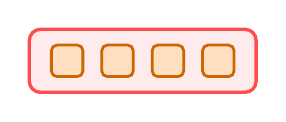
\begin{tikzpicture}[scale=0.8]
  \draw[fill=red!8, draw=red!70, line width=1.2pt, rounded corners=4pt] (-1.8,-0.45) rectangle (1.8,0.55);
  \foreach \x in {-1.2, -0.4, 0.4, 1.2} {
    \draw[fill=orange!25, draw=orange!80!black, line width=1pt, rounded corners=2pt] (\x-0.25,-0.2) rectangle (\x+0.25,0.3);
  }
\end{tikzpicture}
&
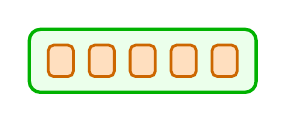
\begin{tikzpicture}[scale=0.8]
  \draw[fill=green!8, draw=green!70!black, line width=1.2pt, rounded corners=4pt] (-1.8,-0.45) rectangle (1.8,0.55);
  \foreach \x in {-1.3, -0.65, 0, 0.65, 1.3} {
    \draw[fill=orange!25, draw=orange!80!black, line width=1pt, rounded corners=2pt] (\x-0.2,-0.2) rectangle (\x+0.2,0.3);
  }
\end{tikzpicture} \\[4pt]
{\bfseries\color{red!85!black} Đĩa đỏ (4 cái bánh)} & {\bfseries\color{green!70!black} Đĩa xanh (5 cái bánh)}
\end{tabular}
\end{center}
\choice
{Đĩa đỏ nhiều hơn đĩa xanh}
{\True Đĩa đỏ ít hơn đĩa xanh}
{Hai đĩa bằng nhau}
{Đĩa xanh ít hơn đĩa đỏ}
\loigiai{
Đĩa đỏ có 4 cái bánh, Đĩa xanh có 5 cái bánh. Vì $4 < 5$ nên \textbf{đĩa đỏ ít hơn đĩa xanh}.\\
\textbf{Đáp án của câu hỏi là B}
}
\end{ex}

% --- CÂU 12 ---
\begin{ex} %[1D1C03]
Trong các nhóm đồ vật dưới đây, nhóm nào có số lượng \textbf{nhiều nhất}?
\choice
{Nhóm 3 quả bóng}
{\True Nhóm 6 bông hoa}
{Nhóm 4 cái bút}
{Nhóm 2 ngôi sao}
\loigiai{
So sánh các số lượng: $6 > 4 > 3 > 2$.\\
Nhóm có số lượng nhiều nhất là \textbf{nhóm 6 bông hoa}.\\
\textbf{Đáp án của câu hỏi là B}
}
\end{ex}

\newpage
% =========================================================================
% PHẦN 2: TRẮC NGHIỆM ĐÚNG SAI (QUAN SÁT TRANH MINH HỌA)
% =========================================================================
\textbf{Phần 2. Trắc nghiệm đúng sai (Quan sát đồ vật và xét tính đúng/sai)}
\setcounterpageref{ex}{0}

% --- CÂU 13 ---
\begin{ex} %[1D1H03]
Quan sát đồ vật chuẩn bị cho bữa tiệc sinh nhật:
\begin{center}
\begin{tabular}{cc}
\begin{tikzpicture}[scale=0.75]
  \draw[fill=blue!5, draw=blue!60, line width=1pt, rounded corners=4pt] (-2.2,-0.55) rectangle (2.2,0.55);
  \foreach \x in {-1.6, -0.8, 0, 0.8, 1.6} {
    \draw[fill=cyan!20, draw=blue!80, line width=0.9pt] (\x,0) ellipse (0.32cm and 0.16cm);
  }
  \node[font=\small\bfseries\color{blue!80!black}] at (0, -0.85) {5 chiếc đĩa};
\end{tikzpicture}
&
\begin{tikzpicture}[scale=0.75]
  \draw[fill=teal!5, draw=teal!60, line width=1pt, rounded corners=4pt] (-2.2,-0.55) rectangle (2.2,0.55);
  \foreach \x in {-1.6, -0.8, 0, 0.8, 1.6} {
    \VeChiecThia{\x}{0.05}
  }
  \node[font=\small\bfseries\color{teal!80!black}] at (0, -0.85) {5 chiếc thìa};
\end{tikzpicture} \\[16pt]
\begin{tikzpicture}[scale=0.75]
  \draw[fill=orange!5, draw=orange!60, line width=1pt, rounded corners=4pt] (-2.2,-0.55) rectangle (2.2,0.55);
  \foreach \x in {-1.1, 0, 1.1} {
    \VeCocNuoc{\x}{0.05}
  }
  \node[font=\small\bfseries\color{orange!90!black}] at (0, -0.85) {3 cốc nước};
\end{tikzpicture}
&
\begin{tikzpicture}[scale=0.75]
  \draw[fill=red!5, draw=red!60, line width=1pt, rounded corners=4pt] (-2.2,-0.55) rectangle (2.2,0.55);
  \foreach \x in {-1.6, -1.0, -0.3, 0.3, 1.0, 1.6} {
    \VeDauTay{\x}{0.05}
  }
  \node[font=\small\bfseries\color{red!80!black}] at (0, -0.85) {6 quả dâu tây};
\end{tikzpicture}
\end{tabular}
\end{center}
Xét tính đúng sai của các câu sau:
\choiceTF
{\True Số đĩa bằng số thìa}
{\True Số cốc nước ít hơn số đĩa}
{Số quả dâu ít hơn số cốc nước}
{\True Nhóm quả dâu tây có số lượng nhiều nhất}
\loigiai{
\begin{itemize}
    \item Số đĩa bằng số thìa ($5 = 5$): \textbf{Đúng}.
    \item Cốc nước (3) ít hơn đĩa (5): \textbf{Đúng}.
    \item Quả dâu (6) nhiều hơn cốc nước (3), nói ít hơn là: \textbf{Sai}.
    \item Quả dâu tây có 6 quả, là nhiều nhất: \textbf{Đúng}.
\end{itemize}
}
\end{ex}

% --- CÂU 14 ---
\begin{ex} %[1D1V03]
Quan sát vườn hoa xinh xắn:
\begin{center}
\begin{tabular}{ccc}
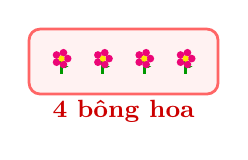
\begin{tikzpicture}[scale=0.75]
  \draw[fill=red!5, draw=red!60, line width=1pt, rounded corners=4pt] (-1.6,-0.55) rectangle (1.6,0.55);
  \foreach \x in {-1.05, -0.35, 0.35, 1.05} {
    \VeBongHoa{\x}{0.05}
  }
  \node[font=\small\bfseries\color{red!80!black}] at (0, -0.85) {4 bông hoa};
\end{tikzpicture}
&
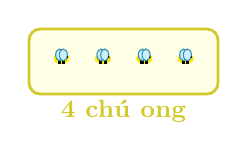
\begin{tikzpicture}[scale=0.75]
  \draw[fill=yellow!10, draw=yellow!80!black, line width=1pt, rounded corners=4pt] (-1.6,-0.55) rectangle (1.6,0.55);
  \foreach \x in {-1.05, -0.35, 0.35, 1.05} {
    \VeChuOng{\x}{0.05}
  }
  \node[font=\small\bfseries\color{yellow!80!black}] at (0, -0.85) {4 chú ong};
\end{tikzpicture}
&
\begin{tikzpicture}[scale=0.75]
  \draw[fill=purple!5, draw=purple!60, line width=1pt, rounded corners=4pt] (-1.4,-0.55) rectangle (1.4,0.55);
  \foreach \x in {-0.6, 0.6} {
    \VeChuBuom{\x}{0.05}
  }
  \node[font=\small\bfseries\color{purple!80!black}] at (0, -0.85) {2 chú bướm};
\end{tikzpicture}
\end{tabular}
\end{center}
Xét tính đúng sai của các câu sau:
\choiceTF
{\True Số hoa đỏ bằng số chú ong}
{\True Số chú bướm ít hơn số chú ong}
{Số chú bướm nhiều hơn số hoa đỏ}
{\True Số hoa đỏ nhiều hơn số chú bướm}
\loigiai{
\begin{itemize}
    \item Hoa đỏ bằng chú ong ($4 = 4$): \textbf{Đúng}.
    \item Bướm (2) ít hơn ong (4): \textbf{Đúng}.
    \item Bướm ít hơn hoa đỏ, nói nhiều hơn là: \textbf{Sai}.
    \item Hoa đỏ (4) nhiều hơn bướm (2): \textbf{Đúng}.
\end{itemize}
}
\end{ex}

% =========================================================================
% PHẦN 3: TRẢ LỜI NGẮN (ĐIỀN SỐ THÍCH HỢP VÀO Ô TRỐNG)
% =========================================================================
\textbf{Phần 3. Trả lời ngắn (Quan sát hình vẽ và điền số thích hợp)}
\setcounterpageref{ex}{0}

% --- CÂU 15 ---
\begin{ex} %[1D1H03]
Có $4$ chú mèo và $4$ con cá. Nối mỗi chú mèo với một con cá thì còn thừa mấy con cá?
\begin{center}
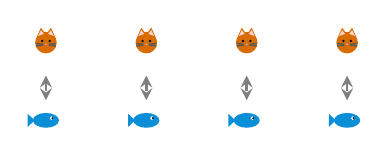
\begin{tikzpicture}[scale=0.85, baseline=(current bounding box.center)]
  \foreach \x in {-2.25, -0.75, 0.75, 2.25} {
    \VeChuMeo{\x}{0.6}
    \draw[<->, >=stealth, dashed, line width=0.9pt, gray] (\x, 0.22) -- (\x, -0.15);
    \VeConCa{\x}{-0.45}
  }
\end{tikzpicture}
\end{center}
\shortans{0}
\loigiai{
\textbf{Đáp số:} $0$\\
Số mèo bằng số cá ($4 = 4$) nên còn thừa $0$ con cá.
}
\end{ex}

% --- CÂU 16 ---
\begin{ex} %[1D1H03]
Có $5$ chiếc ghế và $6$ bạn nhỏ. Mỗi bạn ngồi một ghế thì còn thiếu mấy chiếc ghế?
\begin{center}
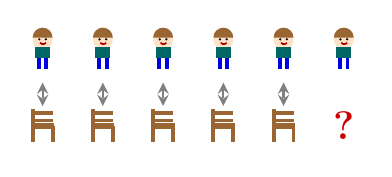
\begin{tikzpicture}[scale=0.85, baseline=(current bounding box.center)]
  \foreach \x in {-2.25, -1.35, -0.45, 0.45, 1.35, 2.25} {
    \VeBanNho[teal!80!black]{\x}{0.5}
  }
  \foreach \x in {-2.25, -1.35, -0.45, 0.45, 1.35} {
    \draw[<->, >=stealth, dashed, line width=0.8pt, gray] (\x, 0.2) -- (\x, -0.15);
    \VeChiecGhe{\x}{-0.45}
  }
  \node[font=\bfseries\Large\color{red!80!black}] at (2.25, -0.45) {?};
\end{tikzpicture}
\end{center}
\shortans{1}
\loigiai{
\textbf{Đáp số:} $1$\\
$6 - 5 = 1$. Còn thiếu $1$ chiếc ghế.
}
\end{ex}

\newpage
% --- CÂU 17 ---
\begin{ex} %[1D1V03]
Hàng trên có $7$ ngôi sao, hàng dưới có $5$ ngôi sao. Hàng trên nhiều hơn hàng dưới mấy ngôi sao?
\begin{center}
\begin{tikzpicture}[scale=0.75, baseline=(current bounding box.center)]
  \foreach \x in {-3.6, -2.4, -1.2, 0, 1.2, 2.4, 3.6} {
    \node[draw=orange!80!black, fill=yellow!80, star, star points=5, star point ratio=2.2, line width=0.7pt, minimum size=0.6cm] at (\x, 0.5) {};
  }
  \foreach \x in {-3.6, -2.4, -1.2, 0, 1.2} {
    \node[draw=blue!80!black, fill=cyan!60, star, star points=5, star point ratio=2.2, line width=0.7pt, minimum size=0.6cm] at (\x, -0.4) {};
  }
\end{tikzpicture}
\end{center}
\shortans{2}
\loigiai{
\textbf{Đáp số:} $2$\\
$7 - 5 = 2$. Hàng trên nhiều hơn hàng dưới $2$ ngôi sao.
}
\end{ex}

% --- CÂU 18 ---
\begin{ex} %[1D1V03]
Đĩa A có $6$ quả táo, đĩa B có số quả táo \textbf{bằng đĩa A}. Hỏi đĩa B có bao nhiêu quả táo?
\begin{center}
\begin{tabular}{cc}
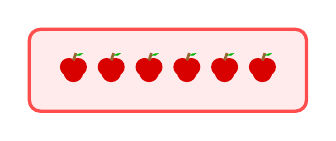
\begin{tikzpicture}[scale=0.8]
  \draw[fill=red!8, draw=red!70, line width=1.2pt, rounded corners=4pt] (-2.2,-0.6) rectangle (2.2,0.7);
  \foreach \x in {-1.5, -0.9, -0.3, 0.3, 0.9, 1.5} {
    \VeQuaTao{\x}{0.05}
  }
\end{tikzpicture}
&
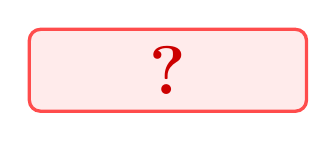
\begin{tikzpicture}[scale=0.8]
  \draw[fill=red!8, draw=red!70, line width=1.2pt, rounded corners=4pt] (-2.2,-0.6) rectangle (2.2,0.7);
  \node[font=\bfseries\Huge\color{red!80!black}] at (0, 0.05) {?};
\end{tikzpicture} \\[4pt]
{\bfseries\color{red!85!black} Đĩa A (6 quả táo)} & {\bfseries\color{red!85!black} Đĩa B (bằng Đĩa A: ? quả)}
\end{tabular}
\end{center}
\shortans{6}
\loigiai{
\textbf{Đáp số:} $6$\\
Vì hai đĩa bằng nhau nên đĩa B cũng có $6$ quả táo.
}
\end{ex}

% --- CÂU 19 ---
\begin{ex} %[1D1V03]
Có $8$ bạn nhỏ đi chơi nhưng chỉ có $5$ chiếc ô che nắng. Có bao nhiêu bạn chưa có ô?
\begin{center}
\begin{tabular}{cc}
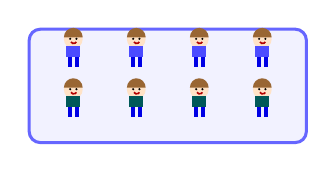
\begin{tikzpicture}[scale=0.8]
  \draw[fill=blue!5, draw=blue!60, line width=1.1pt, rounded corners=4pt] (-2.2,-0.9) rectangle (2.2,0.9);
  \foreach \x in {-1.5, -0.5, 0.5, 1.5} {
    \VeBanNho[blue!70]{\x}{0.4}
    \VeBanNho[teal!70!black]{\x}{-0.4}
  }
\end{tikzpicture}
&
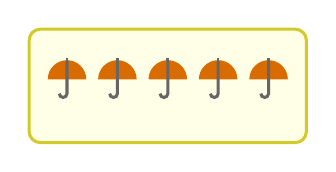
\begin{tikzpicture}[scale=0.8]
  \draw[fill=yellow!10, draw=yellow!80!black, line width=1.1pt, rounded corners=4pt] (-2.2,-0.9) rectangle (2.2,0.9);
  \foreach \x in {-1.6, -0.8, 0, 0.8, 1.6} {
    \VeChiecO[orange!85!black]{\x}{0}
  }
\end{tikzpicture} \\[4pt]
{\bfseries\color{blue!85!black} 8 bạn nhỏ} & {\bfseries\color{yellow!80!black} 5 chiếc ô che nắng}
\end{tabular}
\end{center}
\shortans{3}
\loigiai{
\textbf{Đáp số:} $3$\\
$8 - 5 = 3$. Có $3$ bạn chưa có ô che nắng.
}
\end{ex}

% --- CÂU 20 ---
\begin{ex} %[1D1C03]
Nhóm bông hoa có $9$ bông, nhóm quả táo có $5$ quả. Số bông hoa nhiều hơn số quả táo là bao nhiêu?
\begin{center}
\begin{tabular}{cc}
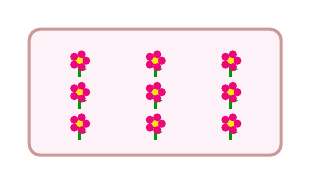
\begin{tikzpicture}[scale=0.8]
  \draw[fill=magenta!5, draw=pink!80!black, line width=1.1pt, rounded corners=4pt] (-2.0,-1.0) rectangle (2.0,1.0);
  \foreach \x/\y in {-1.2/0.5, 0/0.5, 1.2/0.5, -1.2/0, 0/0, 1.2/0, -1.2/-0.5, 0/-0.5, 1.2/-0.5} {
    \VeBongHoa{\x}{\y}
  }
\end{tikzpicture}
&
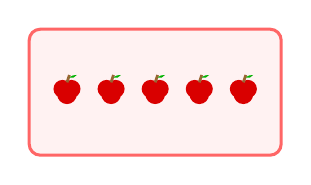
\begin{tikzpicture}[scale=0.8]
  \draw[fill=red!5, draw=red!60, line width=1.1pt, rounded corners=4pt] (-2.0,-1.0) rectangle (2.0,1.0);
  \foreach \x in {-1.4, -0.7, 0, 0.7, 1.4} {
    \VeQuaTao{\x}{0}
  }
\end{tikzpicture} \\[4pt]
{\bfseries\color{magenta!85!black} 9 bông hoa} & {\bfseries\color{red!85!black} 5 quả táo}
\end{tabular}
\end{center}
\shortans{4}
\loigiai{
\textbf{Đáp số:} $4$\\
$9 - 5 = 4$. Số bông hoa nhiều hơn số quả táo là $4$ bông.
}
\end{ex}
